\section{Background}
We first review the the B-Tree data structure, followed by the multi-level parallelism nature of modern SSDs.

\subsection{B-Trees}
B-Trees are a data structure...

\begin{figure}[btree]
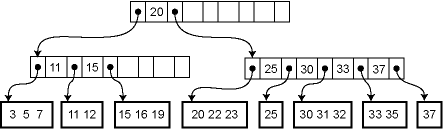
\includegraphics[width=0.45\textwidth]{B-trees.png}
\caption{Standard B-Tree implementation \cite{btrees} with fanout equal to four.}
\label{btree}
\end{figure}

\subsubsection{B-Tree Design and Trade-offs}
B-Trees can be configured in a number of ways. 




\subsection{SSD}

\subsubsection{Multiple Levels of Parallelism in SSDs}

